\documentclass[12pt,a4paper]{report}
\usepackage{amsmath}
\usepackage{amsfonts}
\usepackage{amssymb}
\usepackage{graphicx}
\graphicspath{{images/}}
\usepackage{parskip}
\usepackage{indentfirst}
\usepackage{courier}
\usepackage{titlesec}
\usepackage{wrapfig}
\parindent 15pt
\parskip 2ex

\titleformat{\chapter}[display]   
{\normalfont\huge\bfseries}{\chaptertitlename\ \thechapter}{20pt}{\Huge}   
\titlespacing*{\chapter}{0pt}{-50pt}{20pt}

\author{Jacob Spigle, Zachary Painter, David Akridge, Hunter Figueroa}
\title{Dungeon Master Battle Duels}
\begin{document}
	
\maketitle

\tableofcontents
	
\newpage
\chapter*{Introduction}
\stepcounter{chapter}
\addcontentsline{toc}{chapter}{Introduction}

Role-playing games are games where players act as their characters. Usually in person, around a table, and controlled by the players speaking their actions in turn. This might not always be done by speaking in-character, but rather by following this basic structure:

\begin{enumerate}
	\item The GM describes the environment.
	\item The players describe what they want to do.
	\item The GM narrates the results of the characters? actions.
\end{enumerate}

There are millions of possible character, monster, and scenario possibilities when constructing a tabletop role-playing campaign, however, it is hard and sometimes impossible to sift through them all and find the perfect encounter. Not only that,  but once you commit to a game or role-playing decision you are forced to see it through to completion in order to retain the game?s continuity. Players get one chance to design their character at the very start of a session, and once they do, that character?s path cannot be meaningfully changed. Spending so much time working on a character, and then coming to the first session to find out that they are severely unprepared for the tasks they are presented can be harrowing. On the other side, the GM spends so much time outside of the game to prepare a story and encounters that challenge the Players, so when that GM accidentally wipes out the entire team of Player Characters (PCs) in one unbalanced encounter, or if the PCs simply walk through a fight that was meant to challenge them for the remainder of the session, the GM feels they have failed the PCs in presenting a good game.

\newpage
\chapter*{Proposed Solution}
\stepcounter{chapter}
\addcontentsline{toc}{chapter}{Proposed Solution}

This project presents a service that can be used by both GMs and players to test out their characters, encounters, team builds, or boss fights in a simulated environment. This will allow users to figure out just how well their creation holds up to the requirements that they have set for themselves. This project seeks to develop a service that follows the rules of the d20 Game System, and by allowing the player or GM to import their character's/monsters' statistics and equipment, they then can play against an automated opponent or opponents using that creation. To further enhance a user's ability to test and refine encounters and PCs, users will be able to upload and share their encounters to their public space where others can try their own creations' skills in that creator's setting.

\newpage
\chapter*{Broader Impact}
\stepcounter{chapter}
\addcontentsline{toc}{chapter}{Broader Impact}

Tabletop games bring people together in a world where physical interaction is often lost in lieu of digital communication. This project aims to supplement these interactions by making them more accessible to newer players, as well as help experienced players spend less time on pre-game preparation. This project has the potential to broaden the audience of an already quickly expanding pastime to younger players and DM's. Concepts in the realm of tabletop games are very easily understood by a younger audience, as their imagination and creativity can run free in such games. However, the threshold of understanding for the many rules and balances may prove a bit overzealous for this audience. Having a service that allows improves accessibility to newer players will also bleed into improving accessibility for younger players as well. Additionally, users who do not have a group to play with may find and form groups with other users with whom they have played and shared content with.
	
\newpage
\chapter*{Personal Interests}
\stepcounter{chapter}
\addcontentsline{toc}{chapter}{Personal Interests}
	\section{Jacob Spigle}
	\begin{wrapfigure}{r}{0\textwidth}
		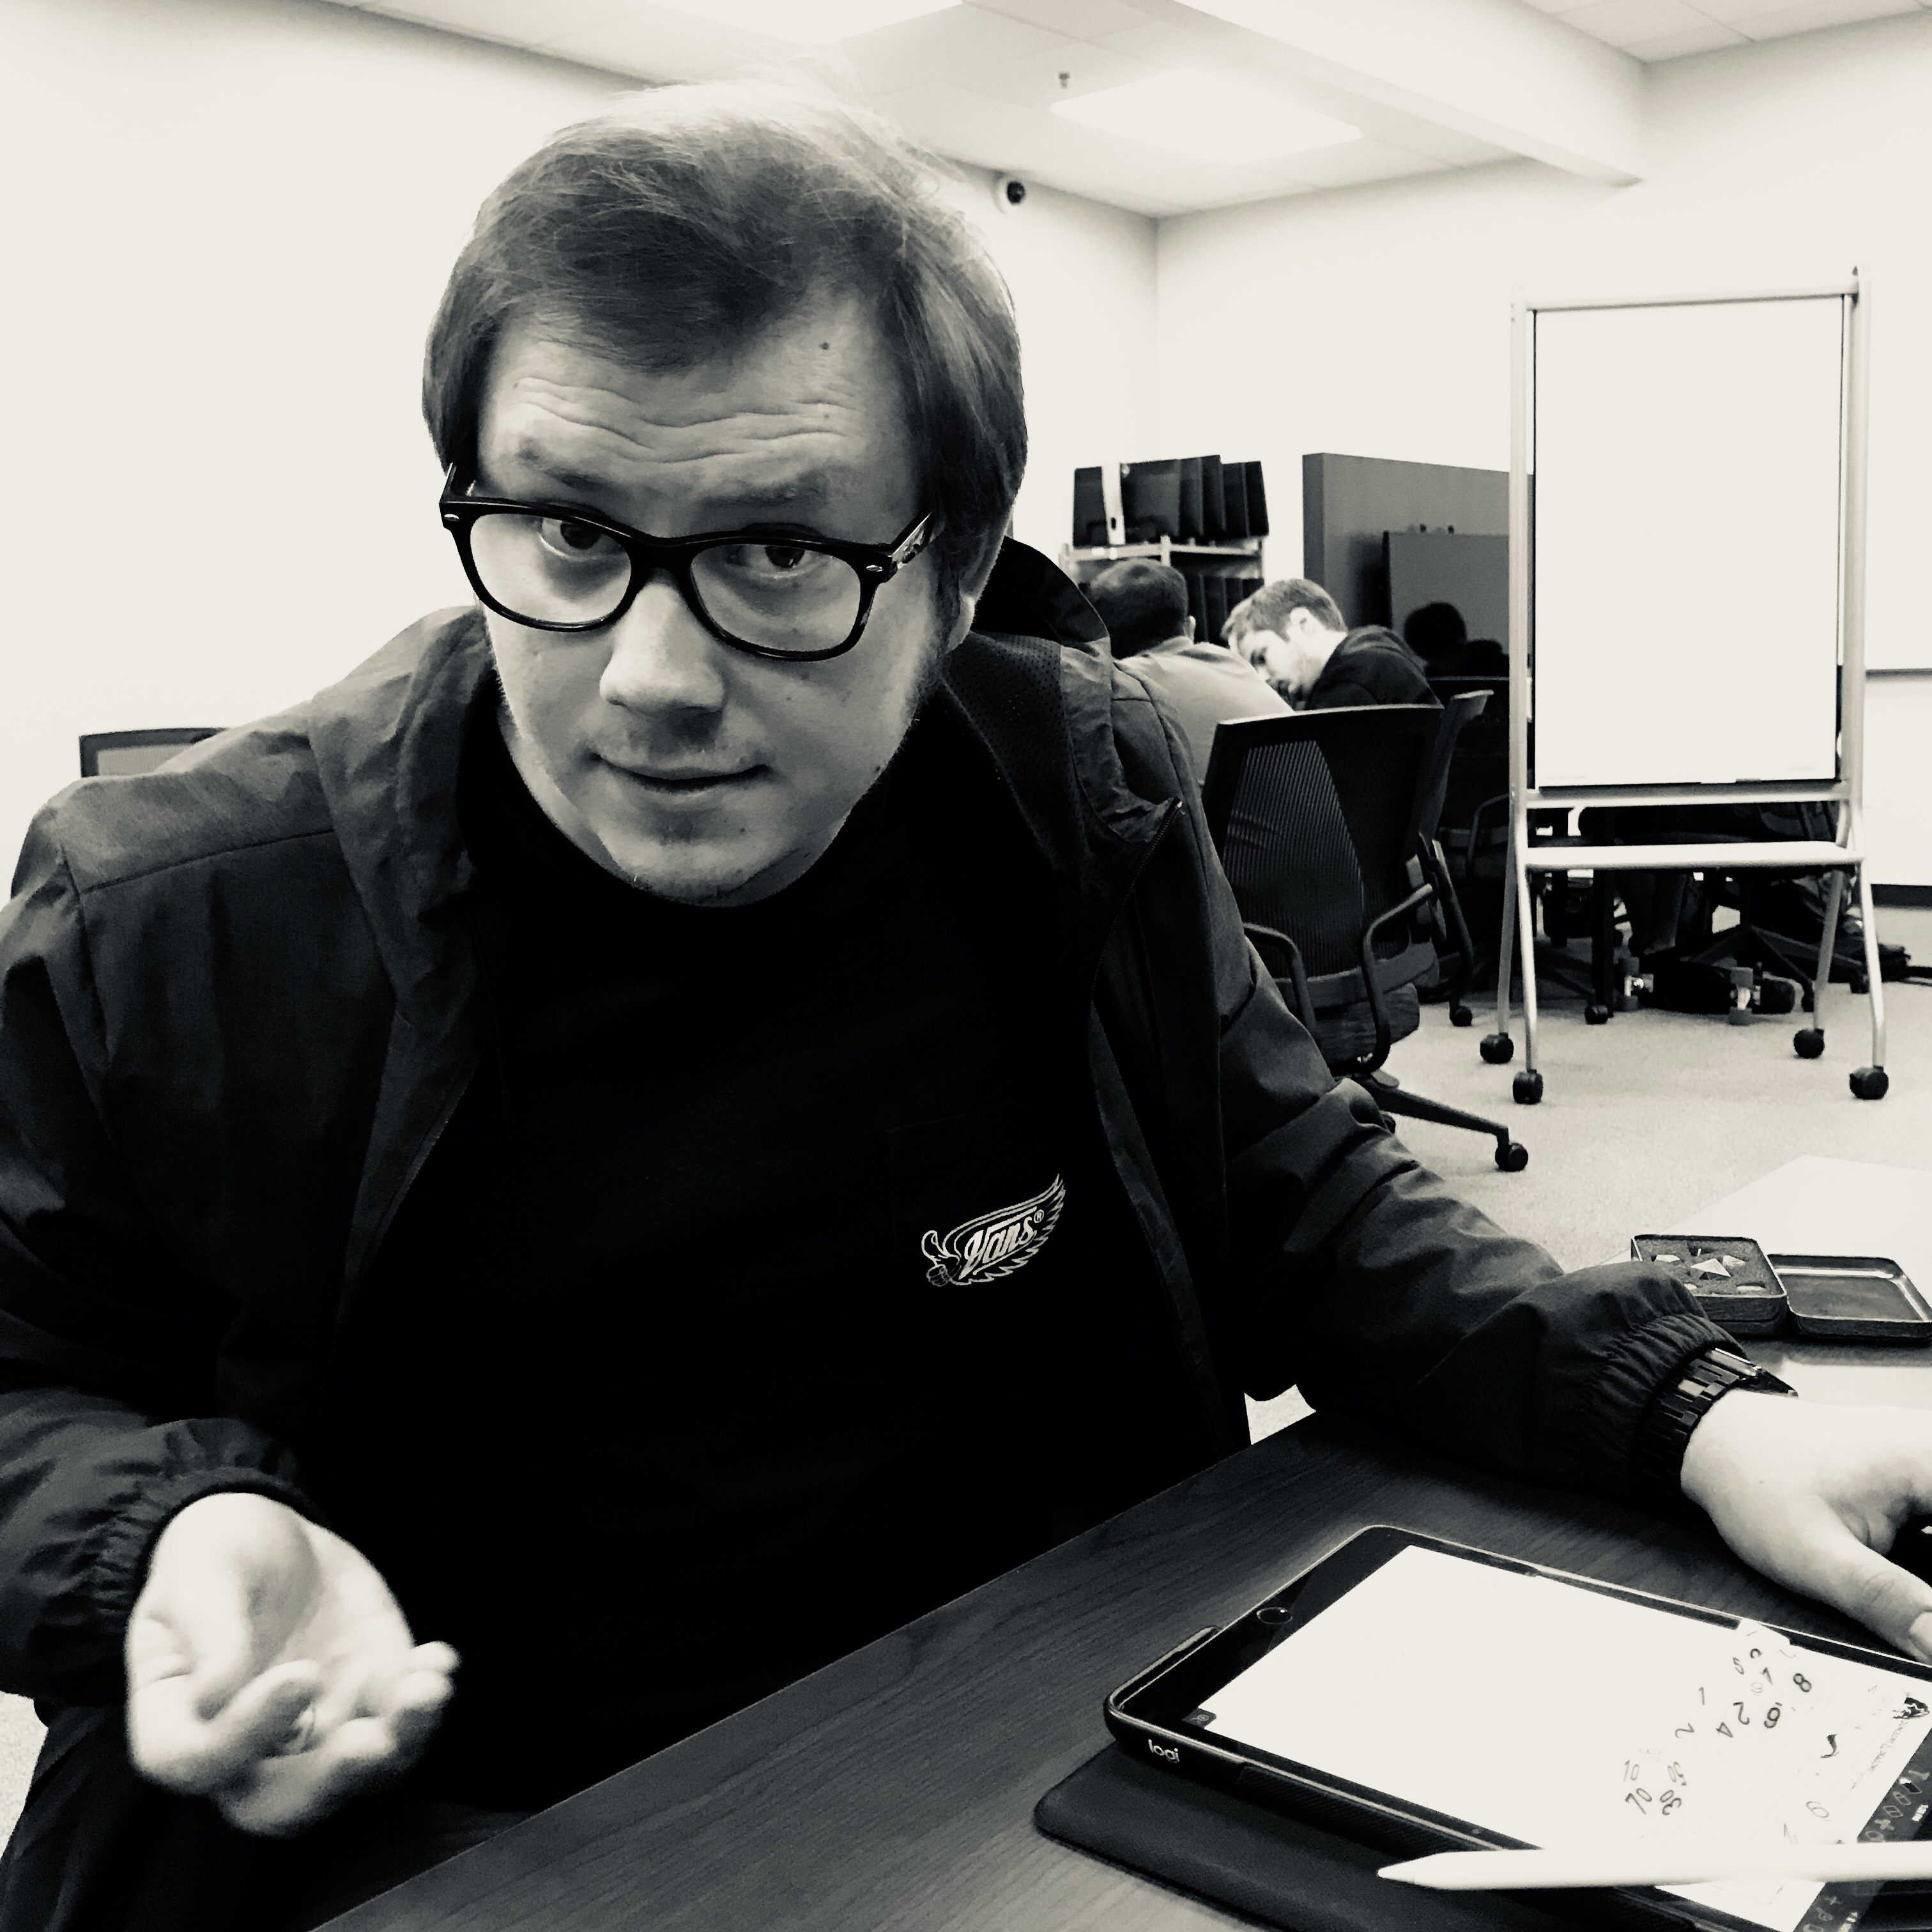
\includegraphics[scale=0.05]{Jacob_Spigle}
	\end{wrapfigure}
	I discovered role-playing games like Dungeons \& Dragons early this year. After playing video games since childhood, D\&D was a breath of fresh air; a way to mix the excitement of creating a character, leveling up, deciding your actions, along with an openness that allows nearly infinite stories, infinite worlds, and the tools to create those stories and worlds yourself. Those infinite possibilities can spur creations that might not work as well in-game as you thought. I have written campaigns and characters that on paper seemed great, but when brought to the table were found lacking. When I searched through the many different forums and groups I had joined after I started playing D\&D, and scouring the internet for a way to playtest my creations, I was surprised to found that no such tool existed. This service is something I can actually use and wish that I had during the creation of campaigns I have written, and that is why I believe others will find use in it as well.
	
	\newpage
	\section{Zachary Painter}
	\begin{wrapfigure}{l}{0\textwidth}
		
\includegraphics[scale=0.05]{Zachary_Painter}
	\end{wrapfigure}
	Some of my primary interests in Computer Science are data structures and algorithms. In my area of research, concurrent programming, these two topics are frequently discussed. Often times in this field, I have had the opportunity to explore many complicated and fascinating algorithms. When tackling these kinds of problems, you often find yourself spending considerably more time thinking and reasoning than implementing/coding. After understanding a problem, you move on to another without getting the chance to apply what you learned in a practical/useable way. This constant cycle of struggle/learn/get-new-problem is something that many students experience throughout college as they rarely have time to stop and demonstrate their rapidly growing skillset in a meaningful way. \par
	My motivation for being part of this project is that I want a chance to slow down and use the skills and algorithms I have picked up in my years at UCF in a useful and creative application instead of an abstract, un-impactful thought exercise. Instead of expecting this project to challenge me with highly complicated algorithms and difficult proofs, I expect this project to challenge me in project management skills, team coding, and the application of numerous techniques that I have learned but never had to implement in a meaningful way. There is an important difference between \textit{knowing} and \textit{doing}; and so I am taking this chance to remind myself what all my learning has amounted to. 
	
	\newpage
	\section{David Akridge}
	\begin{wrapfigure}{r}{0\textwidth}
		
\includegraphics[scale=0.05]{David_Akridge}
	\end{wrapfigure}
	This project caught my interest due to the combination of the creative nature of Dungeons \& Dragons mixed with the real world applications that can be gained by accomplishing the project’s end goal. In my time at UCF, we have learned tons of information primarily focusing on theories and concepts of computer science. While plenty of classes have had us working hands on, there is still much to learn before being able to stand out in the real world. This project is going to have us utilize the various algorithm implementations we’ve learned as well as diving into web development. As we haven’t covered web development in too far detail in the UCF curriculum, this project easily provides an opportunity for me to grasp the understanding of HTML, Javascript, Angular.js, etc. These are all languages and formats that I have had the desire the learn but lacked the drive to do on my own. \par
	Along with being able to learn practical CS skills, DMBD will allow us to find creative workarounds be it code, web-page design, or even artwork. This is a really important aspect of the project to me, because many of the projects we’ve had to do prior have been numerically heavy and honestly not all that interesting. An engaging idea could help propel our ability to learn these new concepts, especially if we are interested in them on our own. Now that there is a great project motivating me and a great team to work alongside with, there is no doubt we will learn all the in’s and out’s of the subject. 
	
	\newpage
	\section{Hunter Figueroa}
	\begin{wrapfigure}{l}{0\textwidth}
		
\includegraphics[scale=0.05]{Hunter_Figueroa}
	\end{wrapfigure}
	I have been playing tabletop role-playing games for over 6 years now. They served as a creative outlet where I could experiment with new creative ideas. I prefer acting as a DM, I’ve only played a single session as a player, I loved the idea of being all powerful creator of a world that I could share with my friends. The tabletop community, namely the Dungeon \& Dragons community is like no other that I have seen before. It is composed of highly talented, highly cooperative  and interactive people who do their very best to better and expand the role playing community. For close to two years now I have put a considerable about of my free time into constructing a digital service to help this same cause. So when I heard Jacob pitch this idea, I knew it was the one for me. We’ve got something really special here, and with the team that we have I feel we can create something game changing.
	
\newpage
\chapter*{User Interface}
\stepcounter{chapter}
\addcontentsline{toc}{chapter}{User Interface}
	\section{Colors}
	\section{Icons}
	\section{Login}
	\section{Register}
	\section{Homepage}
	\section{Search Page}
	\section{Arena Page}
	\section{Battlefield}
	\section{Encounter Profile}
	
\section{User Profile Page}
	
\newpage
\chapter*{Technical Goals}
\stepcounter{chapter}
\addcontentsline{toc}{chapter}{Technical Goals}
	\section{Overall Goals (Requirements???)}
	\section{Project Timelines (Milestones???)}
	\section{Communication}
	\section{Research}
	\section{Budget}

\newpage
\chapter*{Server Design}
\stepcounter{chapter}
\addcontentsline{toc}{chapter}{Server Design}
	\section{User Roles}
	\section{Node.js}
	\section{Express.js}
	\section{Multer}
	\section{Mongoose}
	\section{Server Sequence Diagrams}

\newpage
\chapter*{Database Design}
\stepcounter{chapter}
\addcontentsline{toc}{chapter}{Database Design}
	\section{Schemas}
		\subsection{User Schema}
		\subsection{Arena Schema (HAHA THAT RHYMES)}
		\subsection{Encounter Schema}
		\subsection{Combatant Schema}
		\subsection{Obstacle Schema}

\newpage
\chapter*{Application Design}
\stepcounter{chapter}
\addcontentsline{toc}{chapter}{Application Design}
	\section{Design Patterns}
	\section{Accessibility}
	\section{Types of Views and Controllers}
	\section{In-Game Roles}
	\section{Map / Environments}
	\section{Turn Structure / Order}
	\section{Computer Opponent (A.I.)}
	\section{Encounter Diagnostics (Stress-Tester)}
	\section{Encounter Browser}
	\section{Encounter Creator Tools}
	\section{Storyboards}
	\section{Version Control}
	\section{Data Processing from API (WHAT DOES THIS MEAN???)}

\newpage
\chapter*{Research}
\stepcounter{chapter}
\addcontentsline{toc}{chapter}{Research}
	\section{MEAN Stack}
	The creation of developer tools like MongoDB, Express.js, Angular.js, and Node.js (otherwise known as the MEAN stack) forge a collection of technologies that allow for JavaScript functionality. The culmination of these technologies allow for development of the web application using JavaScript.
		\subsection{Altered MEAN Stack}
		After scouring the internet for alternatives, we found that Meteor.js is a welcome alteration to the MEAN Stack implementation. Meteor.js is another API that allows for focus on JavaScript coding in development across front-end and back-end applications. While it is a bit more heavyweight than the Express.js framework, on the Node.js platform, Meteor.js is designed to accelerate development of web applications. This is achieved by having a number of components pre-configured out-of-the-box, which allows for an enormous head-start in development.
		\subsection{MongoDB}
		\subsection{Meteor.js}
		Meteor.js is a full-stack JavaScript platform for developing modern web and mobile applications. Like much of the API's we are implementing in the development of this web application, Meteor allows for coding in JavaScript across the front-end and back-end side of development. The biggest advocate for including Meteor in our project is its' focus on development speed. The scaffolding that is included directly out of install with Meteor, such as a fully configured MongoDB database and integration with Angular while still having a fully integrated stack, is a leap forward in the development cycle of this project, so we will have more time for fine-tuning features and performance of the web application later. Meteor also uses web sockets instead of HTTP-style pull requests, so the server updates the client when new data is available, and the client renders that data. This allows Meteor to implement "hot-pushing", where developers can push updates the client even while it a user is in the middle of a session. Any fixes or improvements can be pushed without the user even knowing.
		\subsection{Angular 4}
		\subsection{Node.js}
		Node.js is a runtime application that starts small but grows more and more useful as additional modules are implemented. There are a few reasons why it is the first choice when building a web application like this project. Node allows for JavaScript coding on the server side of a website or web application. This results in the idea that code can be written once, but ran on both the server and the client browser, optimizing which functions would give users faster response times while also lifting a bit of work for the server. Writing server-side code in JavaScript using Node also keeps the logic and code very similar across the server and client. Also, Node uses an asynchronous even driven mode, so that when a task is performed, other tasks are not prevented from being run.
		
	\section{Bootstrap 4}
		
	\section{RESTful}
	\section{Game A.I.}
		\subsection{Pathfinding}
		\subsection{Basic Rule Following (Non-A.I. Computer Opponent)}
		\subsection{Decision Trees}

\newpage
\chapter*{Appendix}
\stepcounter{chapter}
\addcontentsline{toc}{chapter}{Appendix}

\newpage
\chapter*{Figures}
\stepcounter{chapter}
\addcontentsline{toc}{chapter}{Figures}

\newpage
\chapter*{Tables}
\stepcounter{chapter}
\addcontentsline{toc}{chapter}{Tables}

\newpage
\chapter*{References}
\stepcounter{chapter}
\addcontentsline{toc}{chapter}{References}
	
\end{document}